\section{Evaluation}
\label{sec:parikshanEvaluation}

To evaluate the performance of \parikshan, we pose and answer the following research questions:

\begin{itemize}
\item \textbf{RQ1:} How long does it take to create a live clone of a production container and what is it's impact on the performance of the production container?\\
\item \textbf{RQ2:} What is the size of the debugging window, and how does it depend on resource constraints?\\ 
\item \textbf{RQ3:} Can we generalize the results of our case study to see if \parikshan can target even more real bugs?
\end{itemize}

We evaluated the \textbf{internal mode} on two identical VM's with an Intel i7 CPU, with 4 Cores, and 16GB RAM each in the same physical host (one each for production and debug containers).
We evaluated the \textbf{external mode} on two identical host nodes with Intel Core 2 Duo Processor, 8GB of RAM.
All evaluations were performed on CentOS 6.5.

%In Section~\ref{sec:performance}, we evaluate live cloning on real-world applications and workloads as well as a micro-benchmark to understand its performance in different scenarios.
%In Section~\ref{sec:timewindowPerformance}, we first provide debug-window sizes for varying workloads run on a live production system. 
%For a more systematic understanding of the debug-window size, we also provide simulation results to show the relationship of buffer overflow with buffer size, the incoming workload, and the instrumentation overhead.
%Finally, in Section~\ref{sec:survey}, we present a survey of 217 real-world bugs, picked from three different applications.
%\xxx{What is the environment we evaluated in? Hardware? Software? Why do we have both real and simulated data?}

\subsection{Live Cloning Performance}
\label{sec:parikshanPerformance}

As explained in Section \ref{sec:design}, a short suspend time during live cloning is necessary to ensure that both containers are in the exact same system state.
The suspend time during live cloning can be divided in 4 parts: 
(1) Suspend \& Dump: time taken to pause and dump the container, 
(2) Pcopy after suspend: time required to complete rsync operation 
(3) Copy Dump File: time taken to copy an initial dump file.
(4) Undump \& Resume: time taken to resume the containers. 
To evaluate ``live cloning'', we ran a micro-benchmark of I/O operations, and evaluated live-cloning on some real-world applications running real-workloads.
\begin{figure}[ht]
  \centering
  \resizebox{.8\linewidth}{!}{
    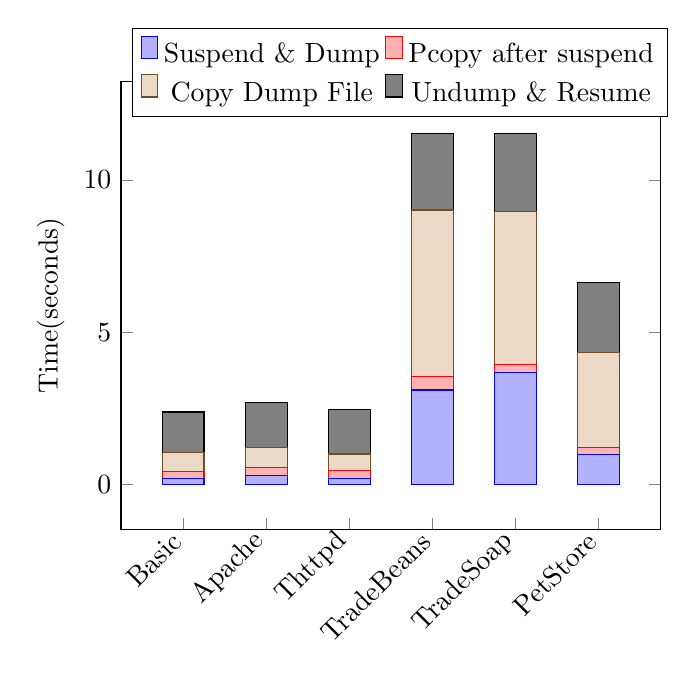
\begin{tikzpicture}
      \begin{axis}[
        ybar stacked,
        bar width=15pt,
        %	nodes near coords,
        enlargelimits=0.15,
        legend style={at={(0.02,1.12)},anchor=north west,legend columns=2},
        ylabel={Time(seconds)},
        symbolic x coords={Basic, Apache, Thttpd, TradeBeans, TradeSoap, 
          PetStore},
        xtick=data,
        x tick label style={rotate=45,anchor=east},
        ]
        \addplot+[ybar] plot coordinates {(Basic,0.21) (Apache,0.30) (Thttpd,0.21) (TradeBeans,3.10) (TradeSoap,3.68) (PetStore,0.97) };
        \addplot+[ybar] plot coordinates {(Basic,0.22) (Apache,0.27) (Thttpd,0.26) (TradeBeans,0.44) (TradeSoap,0.25) (PetStore,0.24) };
        \addplot+[ybar] plot coordinates {(Basic,0.62) (Apache,0.64) (Thttpd,0.53) (TradeBeans,5.47) (TradeSoap,5.03) (PetStore,3.11) };
        \addplot+[ybar] plot coordinates {(Basic,1.33) (Apache,1.47) (Thttpd,1.46) (TradeBeans,2.51) (TradeSoap,2.57) (PetStore,2.32) };
        \addlegendentry{\strut Suspend \& Dump}
        \addlegendentry{\strut Pcopy after suspend}
        \addlegendentry{\strut Copy Dump File}
        \addlegendentry{\strut Undump \& Resume}
      \end{axis}
    \end{tikzpicture}
   }
  %\captionsetup{justification=centering}
  \caption{Suspend time for live cloning, when running a representative benchmark}
  \label{fig:stats}
\end{figure}


\subsubsection{Real world applications and workloads:}
To begin to study the overhead of live cloning, we performed an evaluation using five well-known applications.
Figure~\ref{fig:stats} presents the suspended times for five well-known applications when cloning a replica with \parikshan. 
We ran the httperf~\cite{httperf} benchmark on Apache and \emph{thttpd} to compute max throughput of the web-servers, by sending a large number of concurrent requests.
Tradebeans and Tradesoap are both part of the dacapo~\cite{dacapo} benchmark ``DayTrader'' application.
These are realistic workloads, which run on a multi-tier trading application provided by IBM. 
PetStore~\cite{petstore} is also a well known J2EE reference application. 
We deployed PetStore in a 3-tier system with JBoss, MySQL and Apache servers, and cloned the app-server.
The input workload was a random set of transactions which were repeated for the duration of the cloning process.

As shown in Figure~\ref{fig:stats}, for Apache and Thttpd the container suspend time ranged between 2-3 seconds.
However, in more memory intensive application servers such as PetStore and DayTrader, the total suspend time was higher (6-12 seconds).
Nevertheless, we did not experience any timeouts or errors for the requests in the workload\footnote{In case of packet drops, requests are resent both at the TCP layer, and the application layer. This slows down the requests for the user, but does not drop them}.
However, this did slowdown requests in the workload. 
This shows that short suspend times are largely not visible or have minimal performance impact to the user, as they are within the time out range of most applications.
Further, a clean network migration process ensures that connections are not dropped, and are executed successfully.
We felt that these relatively fast temporary app suspensions were a reasonable price to pay to launch an otherwise overhead-free debug replica.
To further characterize the suspend time imposed by the live cloning phase of \parikshan, we created a synthetic micro-benchmark to push \parikshan towards its limit.

\begin{figure}[ht]
%{0.45\textwidth}
  \centering
  \resizebox{.8\linewidth}{!}{
%\begin{adjustbox}{max size={.9\textwidth}}
    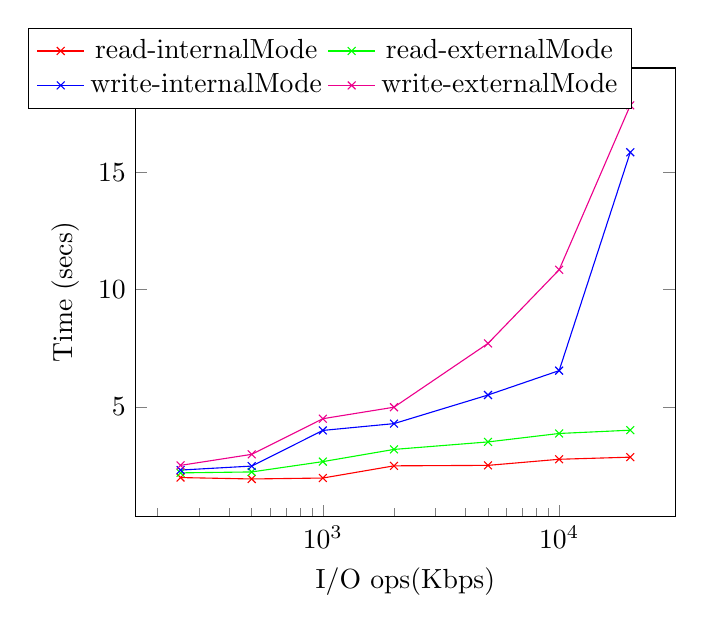
\begin{tikzpicture}
      \begin{axis}[
        xmode=log,
        legend style={at={(-0.2,1.09)},anchor=north west,legend columns=2},
        xlabel=I/O ops(Kbps),
        ylabel=Time (secs)]
        \addplot[color=red,mark=x] coordinates {
          (0,1.85)
          (250,1.99)
          (500,1.93)
          (1000,1.97)
          (2000,2.49)
          (5000,2.51)
          (10000,2.77)
          (20000,2.86)
        };
        \addlegendentry{read-internalMode}
        \addplot[color=green,mark=x] coordinates {
          (0,1.97)
          (250,2.19)
          (500,2.23)
          (1000,2.67)
          (2000,3.19)
          (5000,3.51)
          (10000,3.87)
          (20000,4.01)
        };
        \addlegendentry{read-externalMode}				
        \addplot[color=blue,mark=x] coordinates {
          (0,1.85)
          (250,2.31)
          (500,2.48)
          (1000,4.00)
          (2000,4.29)
          (5000,5.51)
          (10000,6.55)
          (20000,15.86)
        };
        \addlegendentry{write-internalMode}				
        \addplot[color=magenta,mark=x] coordinates {
          (0,1.87)
          (250,2.51)
          (500,2.98)
          (1000,4.50)
          (2000,4.99)
          (5000,7.71)
          (10000,10.85)
          (20000,17.86)
        };
        \addlegendentry{write-externalMode}
      \end{axis}
    \end{tikzpicture}
 % \end{adjustbox}
  }
  %\captionsetup{justification=centering}
  \caption{Live Cloning suspend time with increasing amounts of I/O operations }
  \label{fig:fioResults}
\end{figure}



\subsubsection{Micro Benchmark using I/O operations:}
The main factor that impacts suspend time is the number of ``dirty pages'' in the suspend phase, which have not been copied over in the pre-copy rsync operation (see section~\ref{sec:CloneManager}).
To understand this better, we use \fio (flexible I/O tool for Linux)~\cite{fio}, to gradually increase the number of I/O operations while doing live cloning.
We run the \fio tool to do read and writes of random values with a controlled I/O bandwidth. 
%The suspend time is observed by instrumentation within the cloning script, which reports time taken by each of the suspend processes.
Additionally, we ensure that the I/O job being processed by \fio is long enough to last through the cloning process.

As shown in figure~\ref{fig:fioResults}, read operations have a much smaller impact on suspend time of live cloning compared to write operations.
This can be attributed to the increase of ``dirty pages'' in write operations, whereas for read, the disk image remains largely the same.
The internal mode is much faster than the external mode, as both the production and debug-container are hosted in the same physical device.
We believe, that for higher I/O operations, with a large amount of ``dirty-pages'', network bandwidth becomes a bottleneck: leading to longer suspend times.
Overall in our experiments, the internal mode is able to manage write operation up to 10 Mbps, with a total suspend-time of approx 5 seconds.
Whereas, the external mode is only able to manage up to 5-6 Mbps, for a 5 sec suspend time.\\ \\



\begin{tcolorbox}[breakable, enhanced]
	To answer \textbf{RQ1}, live cloning introduces a short suspend time in the production container dependent on the workload. 
	Write intensive workloads will lead to longer suspend times, while read intensive workloads will take much less. 
	Suspend times in real workload on real-world systems vary from 2-3 seconds for webserver workloads to 10-11 seconds for application/database server workloads. 
	Compared to external mode, internal mode had a shorter suspend time. 
	A production-quality implementation could reduce suspend time further by rate-limiting incoming requests in the proxy, or using copy-on-write mechanisms and faster shared file system/storage devices already available in several existing live migration solutions.
\end{tcolorbox}

\input{parikshan/windowEval}



\subsection{A survey of real-world bugs}
\label{sec:survey}
\noindent

In Table~\ref{tab:survey}, we present the results of a survey of bug reports of three production SOA applications.
In order to understand how we did the survey, let us look at MySQL as an example.
We first searched for bugs which were tagged as ``fixed'' by developers and dumped them.
We then chose a random time-line (2013-2014) and filtered out all bugs which belonged to non-production components - like documentation, installation failure, compilation failure.
We then manually went through each of the bug-reports, filtering out the ones which were mislabeled or were reported based on code-analysis, or did not have a triggering test report (essentially we focused only on bugs that happened during production scenarios).
We then classified these bugs into the categories shown in Table~\ref{tab:survey} based on the bug-report description, and the patch fix, to-do action item for the bug.

One of the core-insights provided by this survey was that most bugs (93\%) triggered in production systems are deterministic in nature (everything but concurrency bugs), among which the most common ones are semantic bugs (80\%).
This is understandable, as they usually happen because of unexpected scenarios or edge cases, that were not thought of during testing.
Recreation of these bugs depend only on the state of the machine, the running environment (other components connected when this bug was triggered), and network input requests, which trigger the bug scenario.
\parikshan is a useful testing tool for testing these deterministic bugs in an exact clone of the production state, with replicated network input. 
The execution can then be traced at a much higher granularity than what would be allowed in production containers, to find the root cause of the bug. 

On the other hand, concurrency errors, which are non-deterministic in nature make up for less than 7\% of the production bugs.
Owing to non-determinism, it is possible that the same execution is not triggered. However concurrent points can still be monitored and a post-facto search of different executions can be done to find the bug~\cite{dpor,systematicDPORconcurrency} to capture these non-deterministic errors.\\ \\


\begin{table}[]
\centering
\begin{tabular}{cccc}
\toprule
\textbf{Category} & \textbf{Apache} & \textbf{MySQL} & \textbf{HDFS} \\ \midrule
\textbf{Performance} & 3 & 10 & 6 \\ 
\textbf{Semantic} & 36 & 73 & 63 \\ 
\textbf{Concurrency} & 1 & 7 & 6 \\ 
\textbf{Resource Leak} & 5 & 6 & 1 \\ \midrule
\textbf{Total} & 45 & 96 & 76 \\
\bottomrule
\end{tabular}
\caption{Survey and classification of bugs}
\label{tab:survey}
\end{table}



\begin{tcolorbox}[breakable, enhanced]
	To answer \textbf{RQ3}, we found that almost 80\% of bugs were semantic in nature, while less than 6\% of the bugs are non-deterministic.
	About 13-14\% of bugs are performance and resource-leak bugs, which are generally persistent in the system.
\end{tcolorbox}
